\documentclass{beamer}\usepackage[]{graphicx}\usepackage[]{color}
%% maxwidth is the original width if it is less than linewidth
%% otherwise use linewidth (to make sure the graphics do not exceed the margin)
\makeatletter
\def\maxwidth{ %
  \ifdim\Gin@nat@width>\linewidth
    \linewidth
  \else
    \Gin@nat@width
  \fi
}
\makeatother

\definecolor{fgcolor}{rgb}{0.345, 0.345, 0.345}
\newcommand{\hlnum}[1]{\textcolor[rgb]{0.686,0.059,0.569}{#1}}%
\newcommand{\hlstr}[1]{\textcolor[rgb]{0.192,0.494,0.8}{#1}}%
\newcommand{\hlcom}[1]{\textcolor[rgb]{0.678,0.584,0.686}{\textit{#1}}}%
\newcommand{\hlopt}[1]{\textcolor[rgb]{0,0,0}{#1}}%
\newcommand{\hlstd}[1]{\textcolor[rgb]{0.345,0.345,0.345}{#1}}%
\newcommand{\hlkwa}[1]{\textcolor[rgb]{0.161,0.373,0.58}{\textbf{#1}}}%
\newcommand{\hlkwb}[1]{\textcolor[rgb]{0.69,0.353,0.396}{#1}}%
\newcommand{\hlkwc}[1]{\textcolor[rgb]{0.333,0.667,0.333}{#1}}%
\newcommand{\hlkwd}[1]{\textcolor[rgb]{0.737,0.353,0.396}{\textbf{#1}}}%
\let\hlipl\hlkwb

\usepackage{framed}
\makeatletter
\newenvironment{kframe}{%
 \def\at@end@of@kframe{}%
 \ifinner\ifhmode%
  \def\at@end@of@kframe{\end{minipage}}%
  \begin{minipage}{\columnwidth}%
 \fi\fi%
 \def\FrameCommand##1{\hskip\@totalleftmargin \hskip-\fboxsep
 \colorbox{shadecolor}{##1}\hskip-\fboxsep
     % There is no \\@totalrightmargin, so:
     \hskip-\linewidth \hskip-\@totalleftmargin \hskip\columnwidth}%
 \MakeFramed {\advance\hsize-\width
   \@totalleftmargin\z@ \linewidth\hsize
   \@setminipage}}%
 {\par\unskip\endMakeFramed%
 \at@end@of@kframe}
\makeatother

\definecolor{shadecolor}{rgb}{.97, .97, .97}
\definecolor{messagecolor}{rgb}{0, 0, 0}
\definecolor{warningcolor}{rgb}{1, 0, 1}
\definecolor{errorcolor}{rgb}{1, 0, 0}
\newenvironment{knitrout}{}{} % an empty environment to be redefined in TeX

\usepackage{alltt}
\usetheme{Madrid}
\usepackage{mathtools}
\usepackage{subfig}
\usepackage{tikz}
\usetikzlibrary{shapes,arrows,positioning}
\pdfmapfile{+sansmathaccent.map}

\AtBeginSection[]{
  \begin{frame}
  \vfill
  \centering
  \begin{beamercolorbox}[sep=8pt,center,shadow=true,rounded=true]{title}
    \usebeamerfont{title}\insertsectionhead\par%
  \end{beamercolorbox}
  \vfill
  \end{frame}
}
%----------------------------------------------------------------------------------------
%	TITLE PAGE
%----------------------------------------------------------------------------------------
\title[decision trees and noisy labels]{%
Decision trees and ways on removing noisy labels\\
  \large Identify costumers in unsound service models}
% The short title appears at the bottom of every slide, the full title is only on the title page

\author{Yannick Misteli} % Your name
\institute[Julius B{\"a}r] % Your institution as it will appear on the bottom of every slide, may be shorthand to save space
{
Julius B{\"a}r \\ % Your institution for the title page
\medskip
\textit{yannick.misteli@juliusbaer.com} % Your email address
}
\date{\today} % Date, can be changed to a custom date
\IfFileExists{upquote.sty}{\usepackage{upquote}}{}
\begin{document}


%----------------------------------------------------------------------------------------
%	PRESENTATION SLIDES
%----------------------------------------------------------------------------------------
\begin{frame}[fragile]
\titlepage % Print the title page as the first slide



\end{frame}
%------------------------------------------------
\begin{frame}[fragile]
\frametitle{Overview} % Table of contents slide, comment this block out to remove it
\tableofcontents % Throughout your presentation, if you choose to use \section{} and \subsection{} commands, these will automatically be printed on this slide as an overview of your presentation
\end{frame}
%------------------------------------------------
\section{Interpretable Models and general aspects of ML} % Sections can be created in order to organize your presentation into discrete blocks, all sections and subsections are automatically printed in the table of contents as an overview of the talk
%------------------------------------------------


\subsection{Introduction} % A subsection can be created just before a set of slides with a common theme to further break down your presentation into chunks
%------------------------------------------------
\begin{frame}[fragile]
\frametitle{Introduction}
% Define block styles
%\tikzstyle{decision} = [diamond, draw, fill=blue!20, 
 %   text width=4.5em, text badly centered, node distance=1.5cm, inner sep=0pt]
\tikzstyle{block} = [rectangle, draw, fill=blue!50, 
    text width=4em, text centered, rounded corners, minimum height=2em]
\tikzstyle{line} = [draw, -latex']
\tikzstyle{cloud} = [draw, ellipse,fill=blue!20, node distance=2cm,
    minimum height=2em]
\begin{minipage}[c]{.5\textwidth} % Left column and width
\begin{figure}
\textbf{Traditional Programming}\par\medskip
\begin{tikzpicture}[auto]
    % Place nodes
    \node [block] (comp) {Computer};
    \node [cloud, above left of = comp] (data) {Data};
    \node [cloud, above right of=comp] (rules) {Rules};   
    \node [cloud, below of=comp] (output) {Output};
    % Draw edges
    \path [line] (rules) -- (comp);
    \path [line] (data) -- (comp);
    \path [line] (comp) -- (output);
\end{tikzpicture}
%\caption{Business Rules are used together with data to produce output}
\end{figure}
\end{minipage}%
\begin{minipage}[c]{.5\textwidth} % Left column and width
\begin{figure}
\textbf{Supervised Machine Learning}\par\medskip
\begin{tikzpicture}[auto]
    % Place nodes
    \node [block] (comp) {Computer};
    \node [cloud, above left of = comp] (data) {Data};
    \node [cloud, above right of=comp] (output) {Output};   
    \node [cloud, below of=comp] (rules) {Rules};
    % Draw edges
    \path [line] (output) -- (comp);
    \path [line] (data) -- (comp);
    \path [line] (comp) -- (rules);
\end{tikzpicture}
%\caption{The output together with the data is used to deduce business rules.}
\end{figure}
\end{minipage}
\end{frame}

%------------------------------------------------
%
\subsection{Interpretability} % A subsection can be created just before a set of slides with a common theme to further break down your presentation into chunks

%------------------------------------------------
\begin{frame}[fragile]
\frametitle{Interpretability}
\begin{block}{Interpretability}
Interpretability is the degree to which a human can understand the cause of a decision\footnotemark
\end{block}
\begin{itemize}
\item The importance of interpretability or \textbf{what vs why and finding meaning in the world} (Regulator)
\item Criteria for interpretability methods or \textbf{intrinsic vs post hoc}
\item Human-friendly explanations or \textbf{what is a good explanation?}
\end{itemize}
\footnotetext{Miller, Tim. 2017. "Explanation in Artificial Intelligence: Insights from the Social Sciences." arXiv Preprint arXiv:1706.07269}
\end{frame}
%------------------------------------------------
\subsection{Interpretable Models} % A subsection can be created just before a set of slides with a common theme to further break down your presentation into chunks
%------------------------------------------------
\begin{frame}[fragile]
\frametitle{Interpretable Models}
\begin{columns}[c] % The "c" option specifies centered vertical alignment while the "t" option is used for top vertical alignment
\column{.35\textwidth} % Left column and width
\begin{block}{Models}
\begin{itemize}
\item Linear models 
\item Logistic regression 
\item Naive Bayes
\item Decision trees 
\item RuleFit\footnotemark
\item k-Nearest Neighbours
\end{itemize}
\end{block}
\column{.65\textwidth} % Left column and width
\footnotesize
\begin{itemize}
\item[] $y_i = \beta_0 + \beta_1 x_{i,1} + \ldots + \beta_p x_{i,p} + \epsilon_i$
\item[] $P(y_i = 1) = \frac{1}{1+exp(-(\beta_0+\beta_1 x_{i,1} + \ldots + \beta_p x_{i,p}))}$
\item[] \begin{equation*}P(C_k \mid x) = \frac{1}{Z} P(C_k) \prod_{i=1}^n P(x_i \mid C_k)\end{equation*}
\item[] 
\begin{figure}
	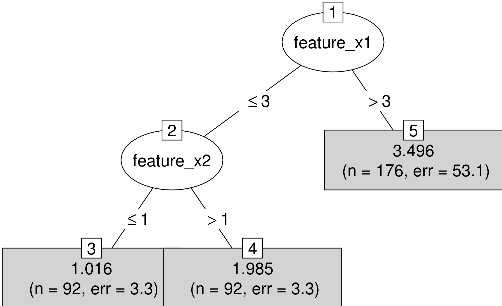
\includegraphics[width=0.5\linewidth]{tree_example.png}
\end{figure}
\item[] 
\begin{figure}
	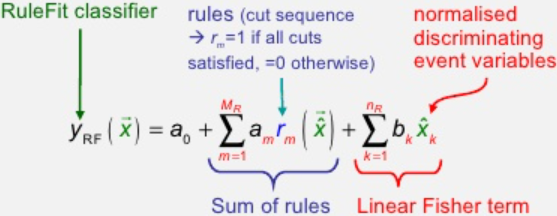
\includegraphics[width=0.6\linewidth]{rulefit.png}
\end{figure}
\item[] \begin{figure}
	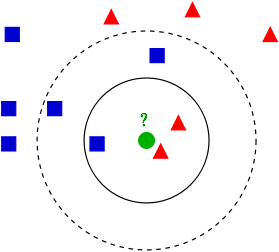
\includegraphics[width=0.15\linewidth]{knn.png}
\end{figure}
\end{itemize}
\end{columns}
\footnotetext{Friedman-Popescu, Tech Rep, Stat. Dpt, Standford U., 2003}
\end{frame}
%------------------------------------------------
\section{Use Case} % A subsection can be created just before a set of slides with a common theme to further break down your presentation into chunks
\subsection{Service Models}
%------------------------------------------------
\begin{frame}[fragile]
\frametitle{Service Models}
\begin{columns}[c] % The "c" option specifies centered vertical alignment while the "t" option is used for top vertical alignment

\column{.45\textwidth} % Left column and width


\textbf{Advisory Service Models}
\begin{enumerate}
\item Basic
\item Premium
\item Advanced
\end{enumerate}

Every advised client signs a service model agreement. Hence, according to preferences and service needs either a basic, premium or advanced service contract is put in place. 

\column{.5\textwidth} % Right column and width

\begin{figure}
	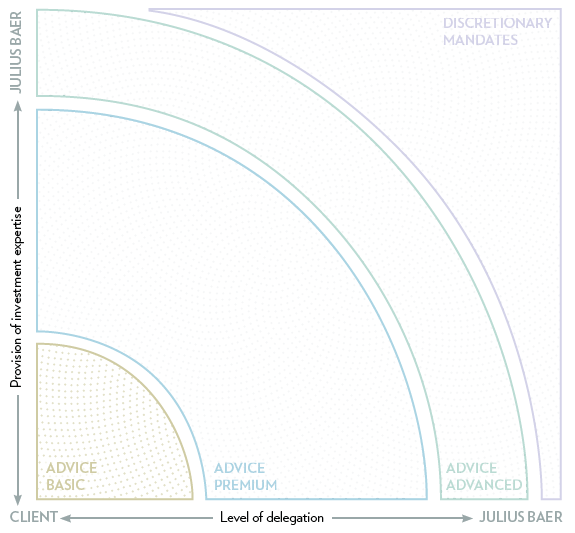
\includegraphics[width=\linewidth]{service_model.png}
\end{figure}

\end{columns}

\begin{figure}
	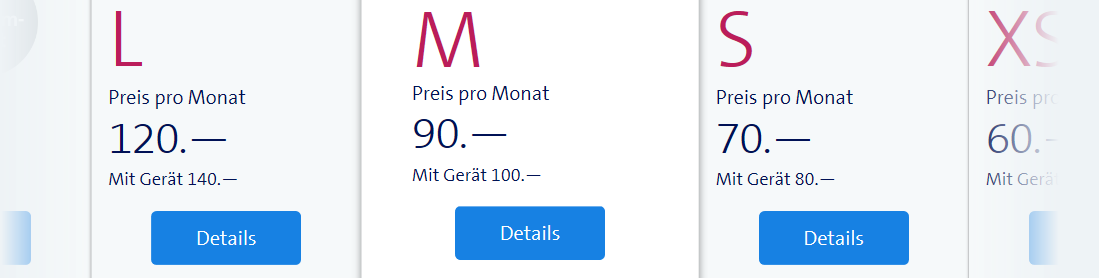
\includegraphics[width=0.5\linewidth]{swisscom.png}
\end{figure}

\end{frame}

\subsection{Use case}
%------------------------------------------------
\begin{frame}[fragile]
\frametitle{Use case}
\begin{columns}[c] % The "c" option specifies centered vertical alignment while the "t" option is used for top vertical alignment
\column{.45\textwidth} % Left column and width
\begin{block}{Problem}
How do identify clients that should be in a different Service Model?
\end{block}
\begin{block}{Idea}
Fit decision tree and investigate terminal nodes for misclassified clients
\end{block}
\column{.5\textwidth} % Right column and width
\begin{figure}
	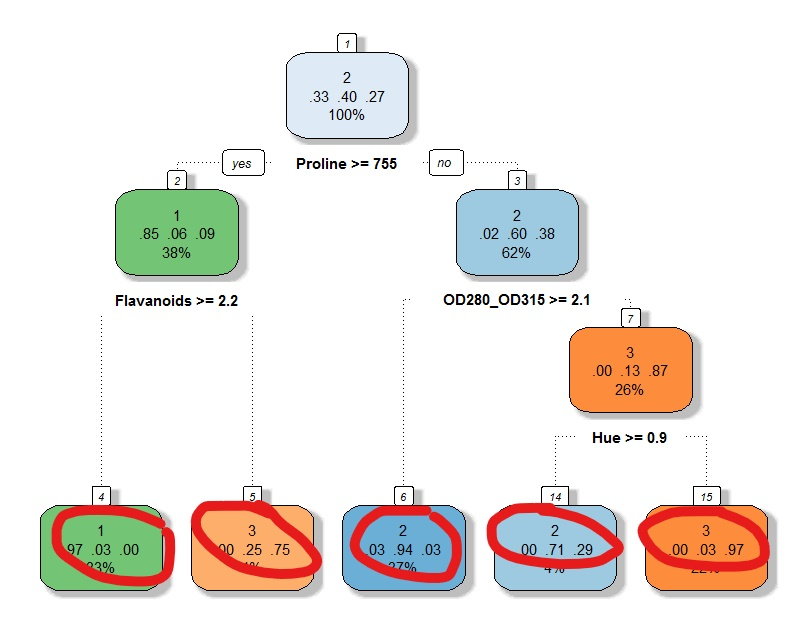
\includegraphics[width=\linewidth]{tree_plot.jpg}
\end{figure}
\end{columns}
\end{frame}

\subsection{Dataset}
%------------------------------------------------
\begin{frame}[fragile]
\frametitle{Dataset}
\small
\begin{columns}[c] % The "c" option specifies centered vertical alignment while the "t" option is used for top vertical alignment
\column{.6\textwidth} % Left column and width
\centering
\begin{block}{Generating multivariate tri-modal mixed distributions}
Multivariate data with count and continouse variable with a pre-specified correlation matrix is generated. The count and continouous variable are assumed to have Poisson and normal marginals, respectively. The resulting mixture is
\centering
\begin{equation*}
F(x) =  \sum_{i=1}^{n}  w_i P_i(x),
\end{equation*}
where $n = 3;w_1 = 0.6, w_2 = 0.3, w_3 = 0.1$ and $P_i$ is the corresponding multivariate Poisson-Normal distribution.
\end{block}
\column{.35\textwidth} % Right column and width
\centering
\begin{figure}
	\includegraphics[width=0.75\linewidth]{multivariate_normal_sample.png}
	\caption{\small Example of sample points from a multivariate normal distribution with $\sigma = \begin{bsmallmatrix} 0 \\ 0 \end{bsmallmatrix}$ and $\Sigma = \begin{bsmallmatrix}1 & \frac{3}{5}\\ \frac{3}{5} & 2\end{bsmallmatrix}$, shown along with the 3-sigma ellipse.\footnotemark}
\end{figure}
\end{columns}
\footnotetext{en.wikipedia.org/wiki/Multivariate\_normal\_distribution}
\end{frame}
%------------------------------------------------
\begin{frame}[fragile]{Data Summary}

\tiny
{\setbeamercolor{block title}{bg=red!75}
\begin{block}{\tiny Syntethic Data}
All data contained in this slides have been generated synthetically and not by Julius B\"{a}r. In no event shall the author or Julius B\"{a}r be liable for any direct, indirect, special or incidental damages resulting from, arising out of or in connection with, the use of the data contained herein.
\end{block}
}
\begin{minipage}[t]{0.45\textwidth}
  \vspace{0pt}

  
\begin{knitrout}
\definecolor{shadecolor}{rgb}{0.969, 0.969, 0.969}\color{fgcolor}\begin{kframe}
\begin{alltt}
\hlkwd{head}\hlstd{(data)}
\end{alltt}
\begin{verbatim}
##   Service.Model Nr.Trades Nr.CCY Nr.Positions
## 1         basic         1      2            1
## 2         basic         2      4            4
## 3      advanced         2      6           15
## 4      advanced         9      6           18
## 5      advanced         2      3            5
## 6       premium         0      3            7
##         AuM       Cash      Random
## 1 1198618.9  133102.70  0.46951209
## 2 1001045.8 -223904.30 -1.18726746
## 3 1629286.8  180392.06  0.54675242
## 4 3947500.7  234791.35  0.01287336
## 5  361907.7  -74267.38 -1.21565020
## 6 2760734.3  340989.71 -2.05284115
\end{verbatim}
\end{kframe}
\end{knitrout}
\end{minipage}
\hfill
\begin{minipage}[t]{0.45\textwidth}
  \vspace{0pt}
\begin{knitrout}
\definecolor{shadecolor}{rgb}{0.969, 0.969, 0.969}\color{fgcolor}\begin{kframe}
\begin{alltt}
\hlkwd{summary}\hlstd{(data[,}\hlnum{1}\hlopt{:}\hlnum{6}\hlstd{])}
\end{alltt}
\begin{verbatim}
##   Service.Model     Nr.Trades     
##  advanced:16955   Min.   : 0.000  
##  basic   :52140   1st Qu.: 1.000  
##  premium :30905   Median : 3.000  
##                   Mean   : 3.394  
##                   3rd Qu.: 4.000  
##                   Max.   :23.000  
##      Nr.CCY        Nr.Positions   
##  Min.   : 1.000   Min.   : 0.000  
##  1st Qu.: 2.000   1st Qu.: 3.000  
##  Median : 3.000   Median : 6.000  
##  Mean   : 3.587   Mean   : 7.478  
##  3rd Qu.: 5.000   3rd Qu.:11.000  
##  Max.   :18.000   Max.   :30.000  
##       AuM                Cash        
##  Min.   :-4851052   Min.   :-464873  
##  1st Qu.:  868542   1st Qu.:   3929  
##  Median : 1385314   Median :  85995  
##  Mean   : 1701572   Mean   : 105146  
##  3rd Qu.: 2346875   3rd Qu.: 183797  
##  Max.   :12001587   Max.   :1066861
\end{verbatim}
\end{kframe}
\end{knitrout}
\end{minipage}
\end{frame}
%------------------------------------------------
\begin{frame}[fragile]{Exploratory Data Analysis}
\tiny

{\setbeamercolor{block title}{bg=red!75}
\begin{block}{\tiny Syntethic Data}
All data contained in this slides have been generated synthetically and not by Julius B\"{a}r. In no event shall the author or Julius B\"{a}r be liable for any direct, indirect, special or incidental damages resulting from, arising out of or in connection with, the use of the data contained herein.
\end{block}
}
\begin{knitrout}
\definecolor{shadecolor}{rgb}{0.969, 0.969, 0.969}\color{fgcolor}
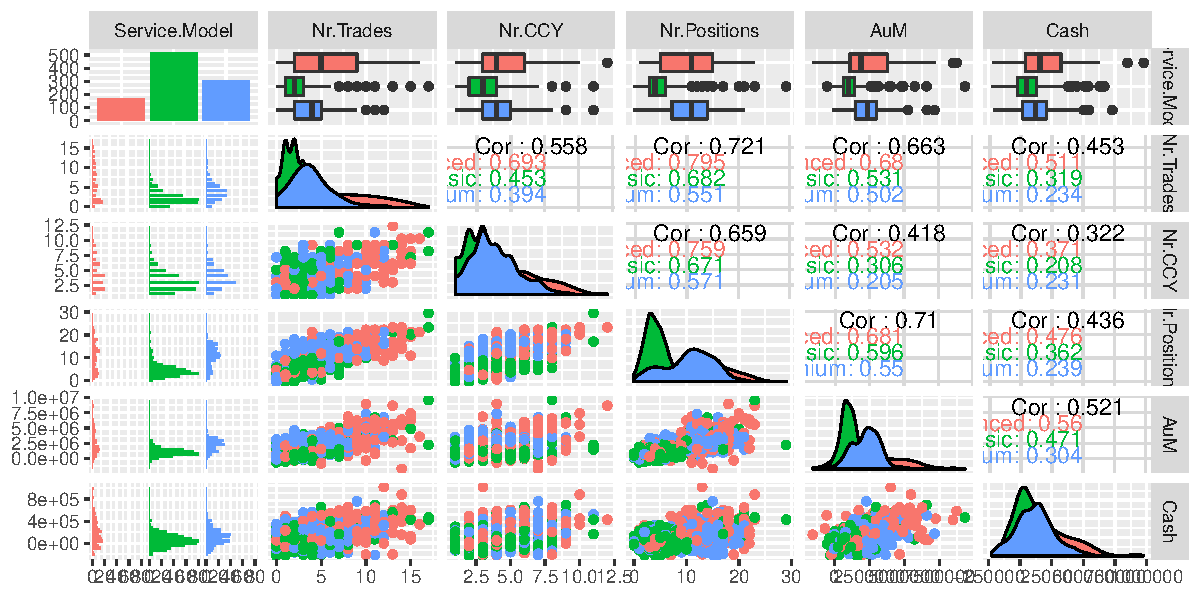
\includegraphics[width=\linewidth]{figure/plots_ggpairs-1} 

\end{knitrout}


\end{frame}
%------------------------------------------------
\begin{frame}[fragile]{Label Noise}
\tiny
{\setbeamercolor{block title}{bg=red!75}
\begin{block}{\tiny Syntethic Data}
All data contained in this slides have been generated synthetically and not by Julius B\"{a}r. In no event shall the author or Julius B\"{a}r be liable for any direct, indirect, special or incidental damages resulting from, arising out of or in connection with, the use of the data contained herein.
\end{block}
}
\begin{knitrout}
\definecolor{shadecolor}{rgb}{0.969, 0.969, 0.969}\color{fgcolor}\begin{kframe}
\begin{alltt}
  \hlstd{noisy_data} \hlkwb{<-} \hlstd{clean_data}
  \hlstd{leng} \hlkwb{<-} \hlkwd{nrow}\hlstd{(noisy_data)}
  \hlstd{labelnoise} \hlkwb{<-} \hlnum{20}
  \hlstd{resample} \hlkwb{<-} \hlkwd{sample.int}\hlstd{(leng, leng}\hlopt{/}\hlnum{100}\hlopt{*}\hlstd{labelnoise)}
  \hlstd{mylabels} \hlkwb{<-} \hlkwd{unique}\hlstd{(clean_data}\hlopt{$}\hlstd{Service.Model)}
  \hlkwa{for}\hlstd{(k} \hlkwa{in} \hlstd{resample)\{}
    \hlstd{myset} \hlkwb{<-} \hlstd{noisy_data[k,]}
    \hlstd{noisy_data[k,}\hlnum{1}\hlstd{]} \hlkwb{<-} \hlkwd{sample}\hlstd{(mylabels[(myset}\hlopt{$}\hlstd{Service.Model} \hlopt{!=} \hlstd{mylabels)],}\hlnum{1}\hlstd{)}
  \hlstd{\}}
\end{alltt}
\end{kframe}
\end{knitrout}
\end{frame}
\subsection{Decision tree}
%------------------------------------------------
\begin{frame}[fragile]{Decision Tree}
\tiny

{\setbeamercolor{block title}{bg=red!75}
\begin{block}{\tiny Syntethic Data}
All data contained in this slides have been generated synthetically and not by Julius B\"{a}r. In no event shall the author or Julius B\"{a}r be liable for any direct, indirect, special or incidental damages resulting from, arising out of or in connection with, the use of the data contained herein.
\end{block}
}
\begin{knitrout}
\definecolor{shadecolor}{rgb}{0.969, 0.969, 0.969}\color{fgcolor}
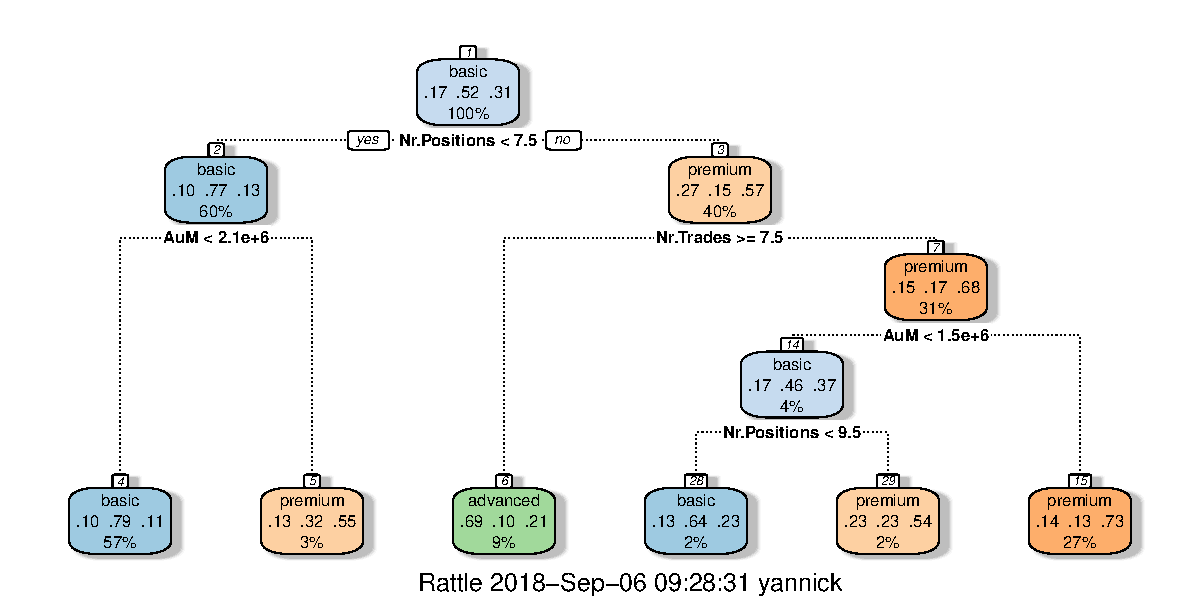
\includegraphics[width=\linewidth]{figure/plots_tree-1} 

\end{knitrout}

\end{frame}

\section{After Math}

\subsection{Noisy Labels}
%------------------------------------------------
\begin{frame}[fragile]{Noisy lables - sources and effects\footnotemark[4]}
\small
\begin{minipage}[c]{0.6\textwidth}
\begin{block}{\small Sources of noise}
\begin{itemize}
\item insufficient information provided to the expert
\item errors in the expert labelling itself
\item subjectivity of the labelling task
\item communication/enconding problems
\end{itemize}
\end{block}
\begin{block}{\small Effects of noise}
\begin{itemize}
\item decrease the classification performances
\item increase/decrease the complexity of learned models
\item pose a threat to tasks like e.g. feature selection
\end{itemize}
\end{block}
\end{minipage}%
\begin{minipage}[c]{0.4\textwidth}
\begin{figure}%
    \centering
    \subfloat{{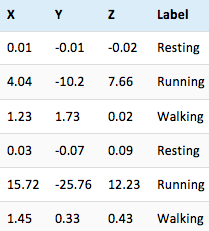
\includegraphics[width=0.3\textwidth]{labels.png} }}%
    \qquad
    \subfloat{{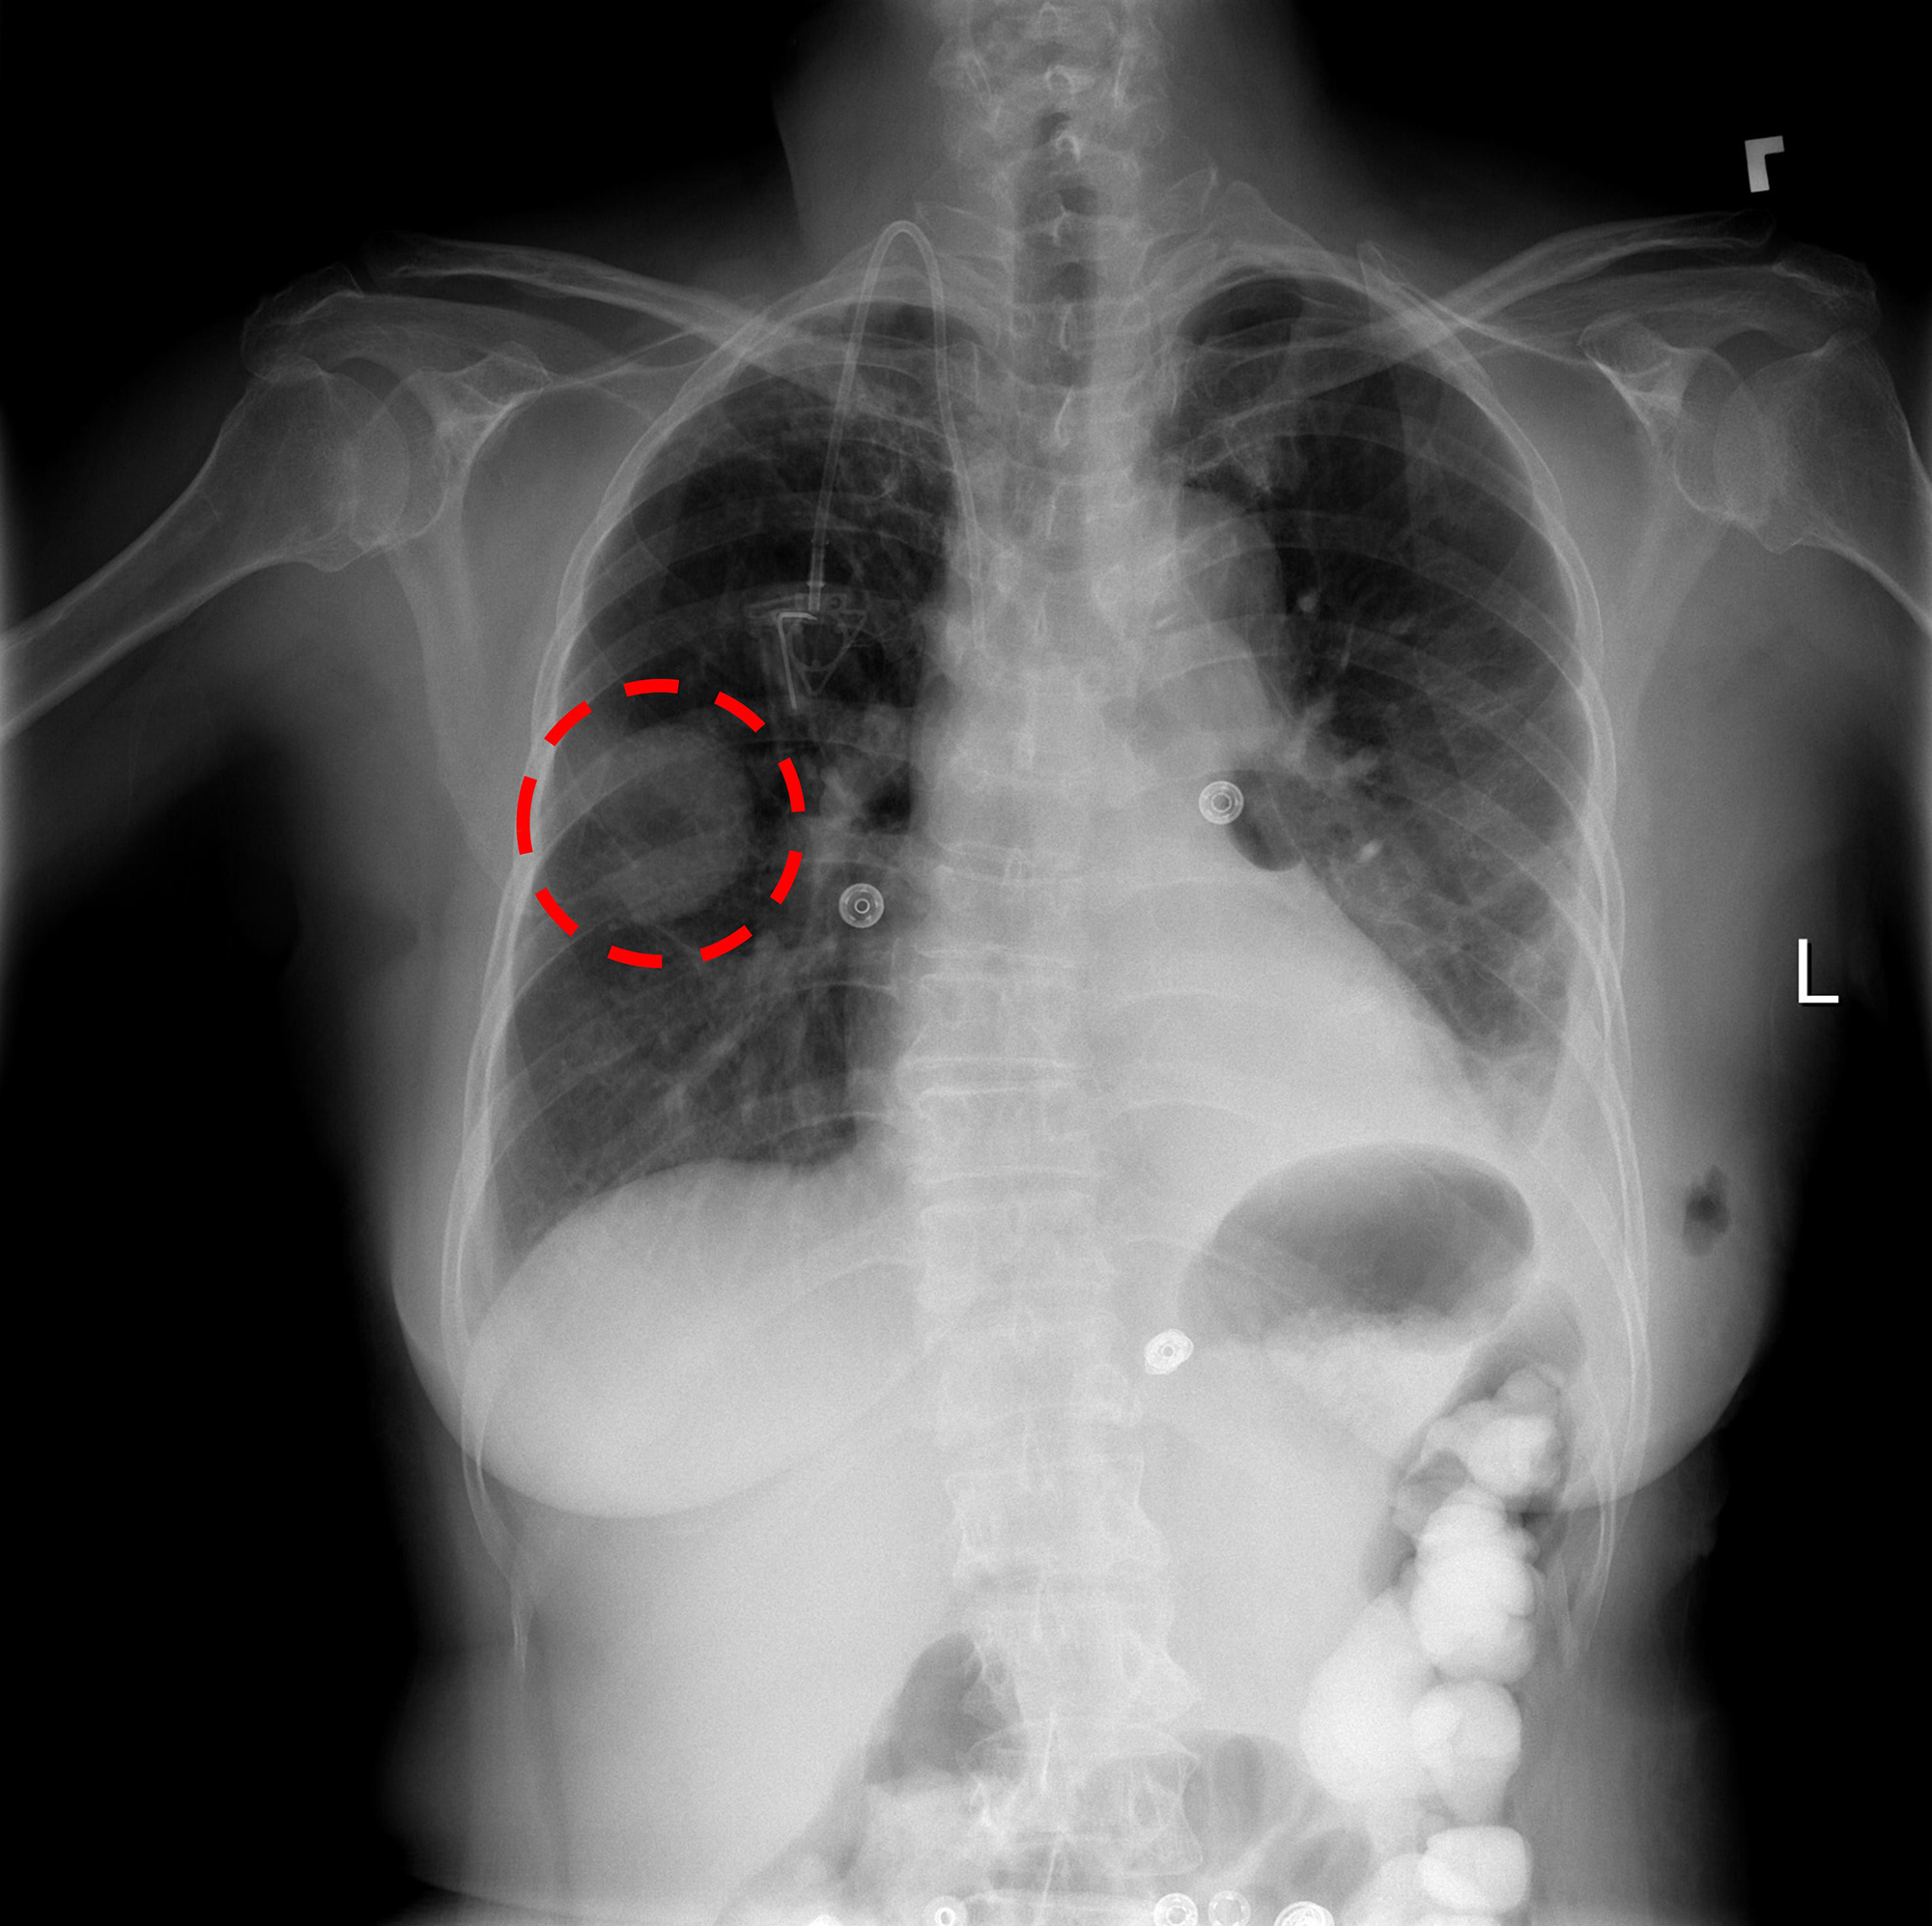
\includegraphics[width=0.3\textwidth]{xray.jpg} }}%
    %\caption{2 Figures side by side}%
    %\label{fig:example}%
\end{figure}
\begin{figure}
	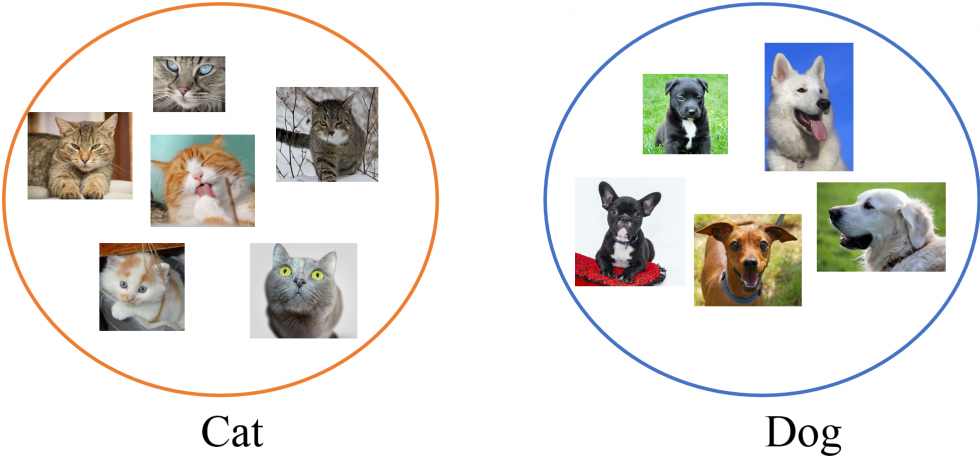
\includegraphics[width=0.75\linewidth]{cat_dog.png}
\end{figure}
\end{minipage}
\footnotetext[4]{\tiny https://labelnoise2017.loria.fr/wp-content/uploads/2017/11/présentation-LABELNOISE17-Frénay.pdf}
\end{frame}

\subsection{Dealing with Noise}
%------------------------------------------------
\begin{frame}[fragile]{Dealing with Noise}
\tiny
\begin{minipage}[c]{0.5\textwidth}
remove
\end{minipage}%
\begin{minipage}[c]{0.5\textwidth}
robust MLS
(SVM soft margin) ensembles
\end{minipage}
\end{frame}

\subsection{Noise Sensitivity of ML algorithms}
%------------------------------------------------
\begin{frame}[fragile]{Noise Sensitivity of ML algorithms}
\tiny
\end{frame}
\end{document}
